%----------------------------------------------------------------------
% Problem 1

\begingroup
\allowdisplaybreaks

\newpage
\section{Problem 1}

\textbf{Exercise 1 in Section 2.7}

\subsection{Solution}
	
\subsubsection{Part A}

The model

\begin{align*}
	t_i = t_0 + s_2 x_i
\end{align*}

can be approached as a discrete linear inverse problem. Six measurements of this system were provided which lead to casting the inverse problem in the form $G\bv{m} = \bv{d}$. The system matrix (i.e., operator) is defined as

\begin{align*}
	G \defeq \begin{bmatrix} 1 & x_1 \\ 1 & x_2 \\ \vdots & \vdots \\ 1 & x_6 \end{bmatrix}
\end{align*}

and data vector simply defined below.

\begin{align*}
	\bv{d} \defeq \begin{bmatrix} t_1 \\ t_2 \\ \vdots \\ t_6 \end{bmatrix}
\end{align*}

Because the standard deviation was provided for the measurement error, a weighted least-squares solution was utilized. Weighting was applied to the operator matrix $G$ and data vector $\bv{d}$ such that:

\begin{align*}
	W = \frac{1}{\sigma} I_6 \\
	\\
	G_w = W G \\
	\\
	\bv{d}_w = W d
\end{align*}

Then, the weighted least-squares solution given as:

\begin{align*}
	\bv{m}_{L2} &= \left(G_w^T G \right)^{-1} G_w^T \bv{d}_{w}
\end{align*}

Using \MATLAB, the solution $\bv{m}_{L2}$ was computed to be:

\begin{align*}
	\bv{m}_{L2} = \begin{bmatrix} t_0 \\ s_2 \end{bmatrix} = \begin{bmatrix} \textrm{2.032337} \\ \textrm{0.220281} \end{bmatrix}
\end{align*}

Figure \ref{fig: prob1 partA} contains the data, the fitted model, and the residuals.

\begin{figure}[h] 
	\centering
	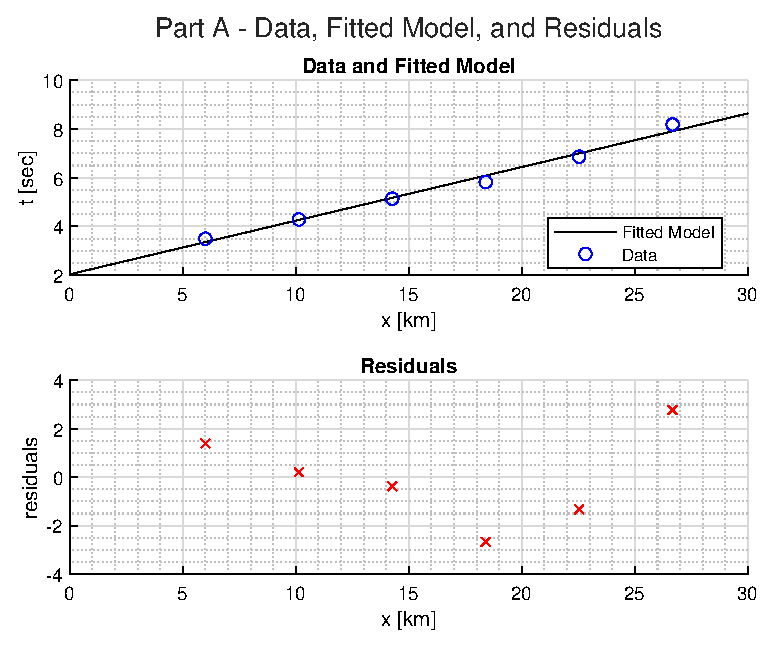
\includegraphics[width=0.8\textwidth]{./images/prob1_partA.eps}
	\caption{Part A - Data, Fitted Model, and Residuals}
	\label{fig: prob1 partA}
\end{figure}
\FloatBarrier


\subsubsection{Part B}

The model covariance matrix $C = \Cov{\bv{m}_{L2}}$ is computed as

\begin{align*}
	A &= \left(G_w^T G \right)^{-1} G_w^T \\
	\\
	C &= A A^T
\end{align*}

Using \MATLAB, the model covariance matrix was computed to be

\begin{align*}
	C = \begin{bmatrix} \textrm{0.01059} & \textrm{-0.0005463} \\ \textrm{-0.0005463} & \textrm{3.3447} \times 10^{-5} \end{bmatrix}
\end{align*}

The model parameter correlation matrix $\rho$ is essentially a scaled version of the model covariance matrix such that

\begin{align*}
	\rho_{m_i,m_j} = \frac{\Cov{m_i,\,m_j}}{\sqrt{\Var{m_i}\Var{m_j}}}
\end{align*}

Using \MATLAB, the model parameter correlation matrix was computed to be

\begin{align*}
	\rho = \begin{bmatrix} \textrm{1} & \textrm{-0.91794} \\ \textrm{-0.91794} & \textrm{1} \end{bmatrix}
\end{align*}

The off-diagonal terms indicate that the two model parameters have a high negative correlation!


\subsubsection{Part C}

The 95\% confidence interval for the model parameters $\bv{m}_{L2}$ given as 

\begin{align*}
	\bv{m}_{L2} \pm \textrm{1.96} \cdot \textrm{diag}\left(C\right)^\frac{1}{2} = \bv{m}_{L2} \pm \begin{bmatrix} \textrm{0.201696} \\ \textrm{0.011335} \end{bmatrix}
\end{align*}

which results in the following 95\% confidence interval which could be interpreted as a box. 

\begin{align*}
	\textrm{1.8306} &\leq t_0 \leq \textrm{2.234} \\
	\\
	\textrm{0.20895} &\leq s_2 \leq \textrm{0.23162}
\end{align*}

However, due to the high correlation between model parameters, interpreting the confidence as a box is insufficient. Instead, the eigenvectors and eigenvalues of $C^{-1}$ are used to form an ellipse which bounds the 95\% confidence interval. The eigenvectors indicate the directions of the semi-major and semi-minor axes, while each axis is scaled by a factor of $\frac{\Delta}{\sqrt{\lambda_i}}$. The region $\Delta^2$ is the inverse $\chi^2$ distribution for a given number of degrees of freedom $\nu$. The degrees of freedom $\nu$ is the number of equations in $G$ (i.e., $m$) minus the number of model parameters $n$. In our case, the number of degrees of freedom is $\nu = m - n = 4$. 

Figure \ref{fig: prob1 partC} shows the comparison between the box interpretation and the ellipse. 

\begin{figure}[h] 
	\centering
	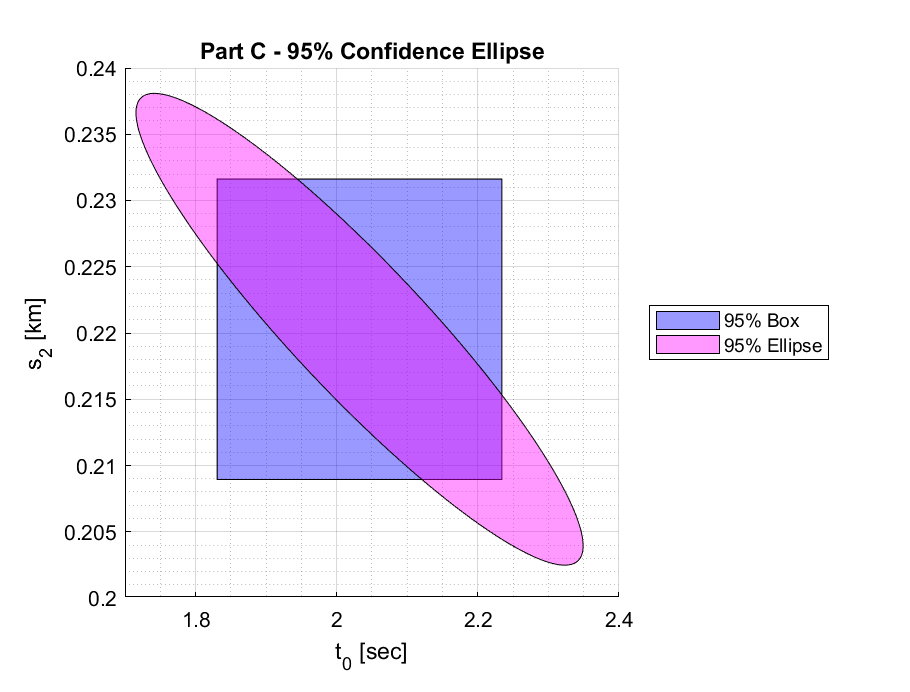
\includegraphics[width=0.8\textwidth]{./images/prob1_partC.eps}
	\caption{Part C - 95\% Confidence Bounds}
	\label{fig: prob1 partC}
\end{figure}
\FloatBarrier


\subsubsection{Part D}

The observed $\chi^2_{obs}$ value is defined as the sum of the residuals when scaled by $\sigma$ such that:

\begin{align*}
	\chi^2_{obs} \defeq \sum_{i=1}^{m} \frac{\left(d_i - \left(G \bv{m}_{L2}\right)_i \right)^2}{\sigma_i^2}
\end{align*}

Then, the p-value is defined as:

\begin{align*}
	p \defeq \int_{\chi^2_{obs}}^{\inf} f_{\chi^2} x dx
\end{align*}

Using \MATLAB, each value was evaluated as:

\begin{align*}
	\chi^2_{obs} &= \textrm{18.750184} \\
	\\
	p &= \textrm{0.000874}
\end{align*}


\subsubsection{Part E}

A Monte-Carlo simulation of 1000 runs was conducted. Figures \ref{fig: prob1 partE 1} and \ref{fig: prob1 partE 2} show histograms for model parameters $t_0$ and $s_2$, as well as the histogram for $chi^2$.

\begin{figure}[h] 
	\centering
	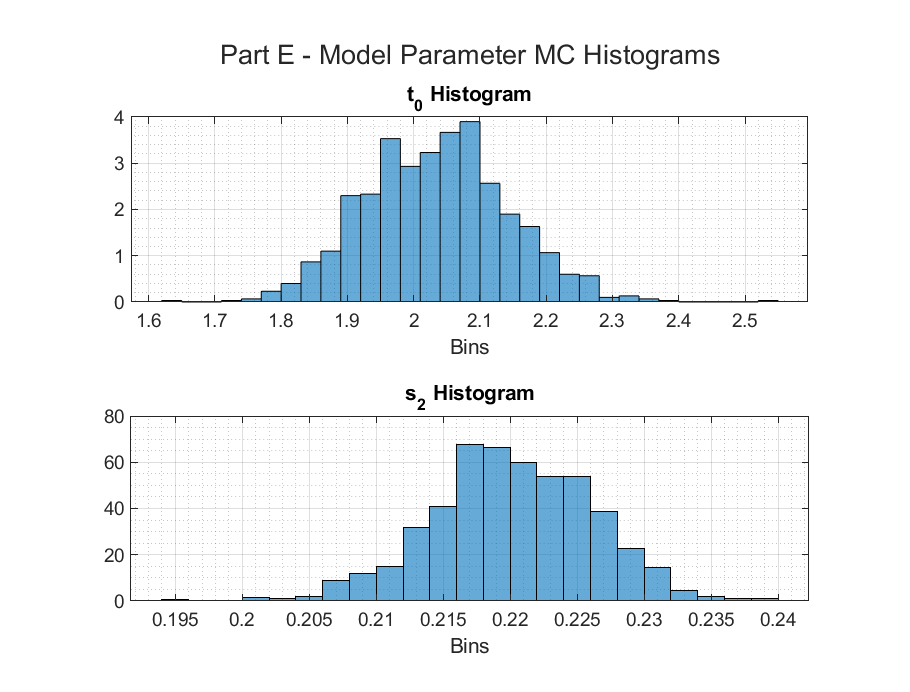
\includegraphics[width=0.8\textwidth]{./images/prob1_partE_1.eps}
	\caption{Part E - Model Parameter Histograms}
	\label{fig: prob1 partE 1}
\end{figure}
\FloatBarrier

\begin{figure}[h] \label
	\centering
	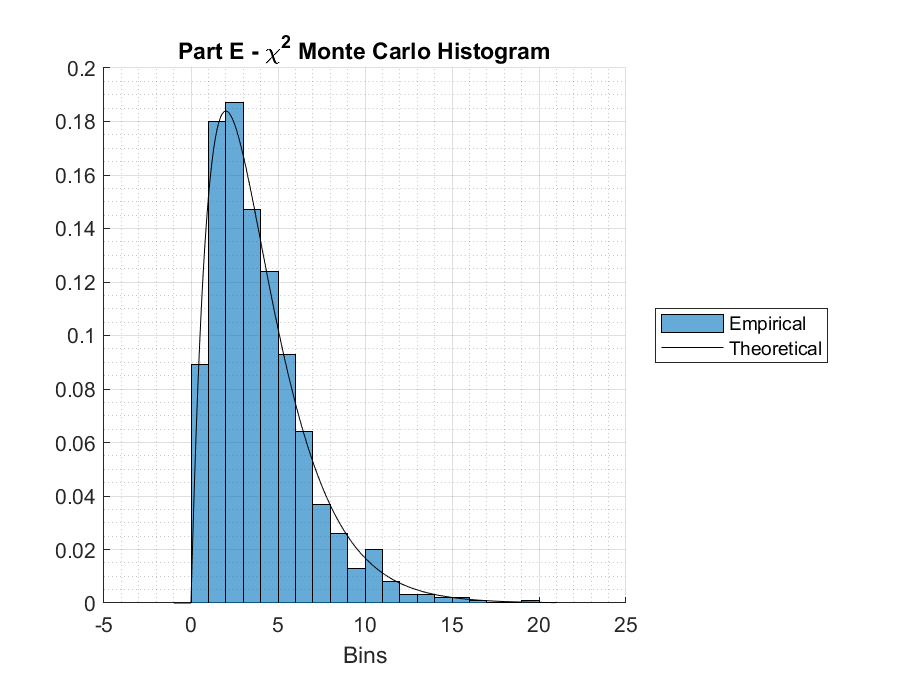
\includegraphics[width=0.8\textwidth]{./images/prob1_partE_2.eps}
	\caption{Part E - $\chi^2$ Histogram}
	\label{fig: prob1 partE 2}
\end{figure}
\FloatBarrier

As expected, the model parameter histograms in figure \ref{fig: prob1 partE 1} appear to be normally distributed, while the $\chi^2$ histogram in figure \ref{fig: prob1 partE 2} appears to keep it's expected shape with a long tail to the right.


\subsubsection{Part F}

First, the Monte-Carlo realizations for the model parameters are consistent with the 95\% confidence ellipse from Part C. 

\begin{figure}[h] 
	\centering
	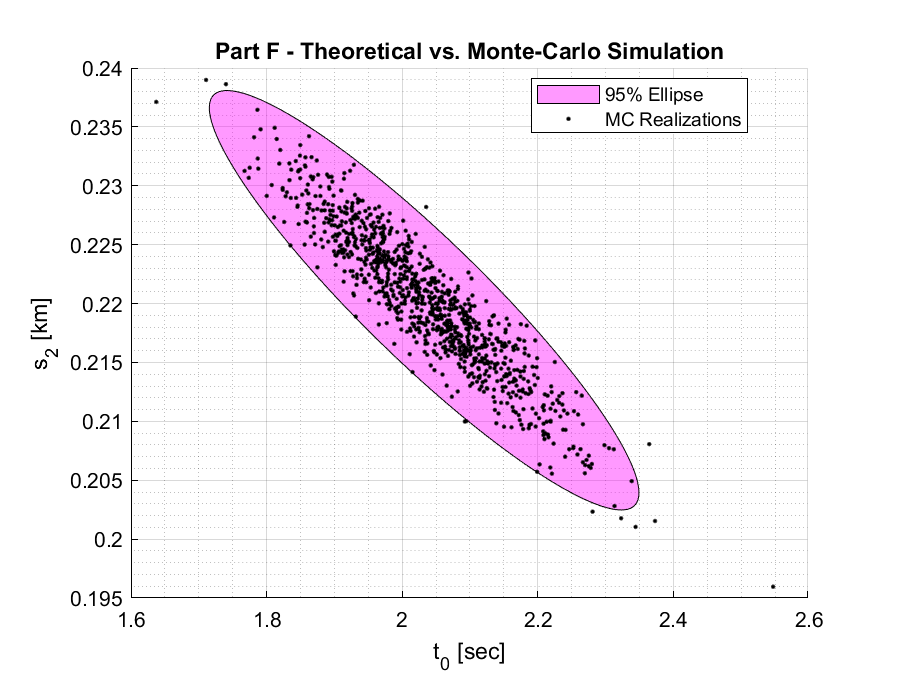
\includegraphics[width=0.8\textwidth]{./images/prob1_partF.eps}
	\caption{Part F - Model Parameter MC Realization vs. 95\% Confidence Ellipse}
	\label{fig: prob1 partF}
\end{figure}
\FloatBarrier

Additionally, there is agreement between the theoretical means of computing $\chi^2_{obs}$ vs. the histogram in figure \ref{fig: prob1 partE 2}. Notice that the mode of the histogram (i.e., bin with the greatest number of occurrences) is near theoretical value of $\chi^2_{obs} = \textrm{18.750184}$. 

I am surprised that with 1000 runs, the two modes are not a closer match. However, I repeated the Monte-Carlo simulation with 100000 runs and got much better agreement. Since I re-seed the random number generator each time the script is called, perhaps I was just "unlucky" and got an unfavorable stochastic run?

Finally, the computed p-value indicates a strong "goodness of fit" measure which is consistent with figure \ref{fig: prob1 partF} which shows that the majority of points are contained within the ellipse. 


\subsubsection{Part G}

L1 regression using iterative reweighted least squares (IRLS) was performed using the same data set. The \verb|irls()| function provided in the \verb|Lib| folder was utilized. This resulted in the following comparison to the L2 regression. 

\begin{figure}[h] 
	\centering
	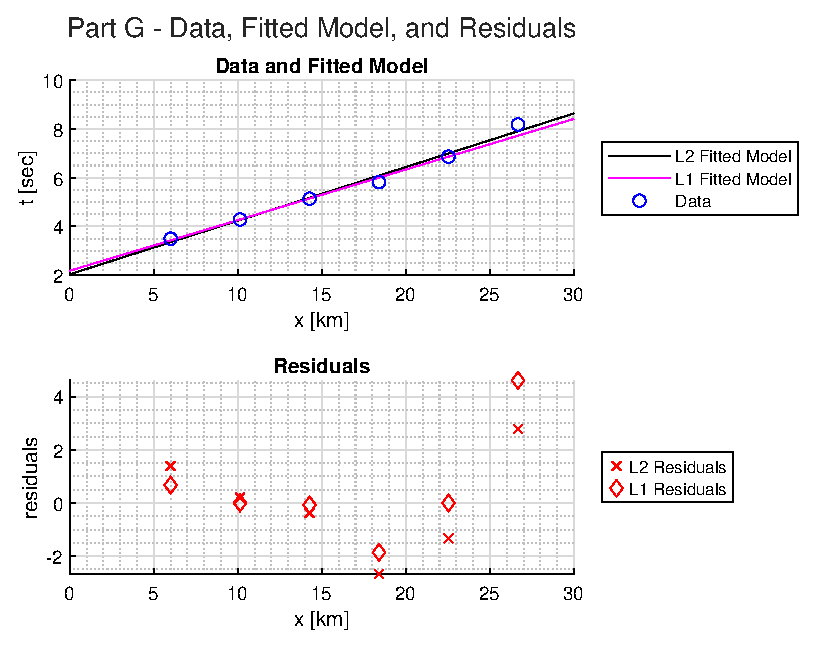
\includegraphics[width=0.8\textwidth]{./images/prob1_partG.eps}
	\caption{Part G - L1 Regression Data, Fitted Model, and Residuals}
	\label{fig: prob1 partG}
\end{figure}
\FloatBarrier


\subsubsection{Part H}

The model covariance resulting from L1 regression was estimated empirically from the 1000 Monte-Carlo trials. With the number of trials $q$, the empirical covariance matrix $C_{L1}$ is computed as

\begin{align*}
	A_{L1} &= \bv{m}_{L1,mc} - \bar{\bv{m}}_{L1,mc} \\
	\\
	C_{L1} &= \frac{A_{L1}^T A_{L1}}{q}
\end{align*}

Using \MATLAB, $C_{L1}$ evaluates to

\begin{align*}
	C_{L1} = \begin{bmatrix} \textrm{0.047204} & \textrm{-0.0019812} \\ \textrm{-0.0019812} & \textrm{9.2902} \times 10^{-5} \end{bmatrix}
\end{align*}

Interestingly enough, the model parameter correlation matrix showed a slightly higher correlation than the L2 regression solution. 

\begin{align*}
	\rho_{L1} = \begin{bmatrix} \textrm{1} & \textrm{-0.9461} \\ \textrm{-0.9461} & \textrm{1} \end{bmatrix}
\end{align*}

When comparing the Monte-Carlo realizations with the resulting 95\% confidence ellipse, there are a few values which fall far outside the ellipse. 

 \begin{figure}[h] 
 	\centering
 	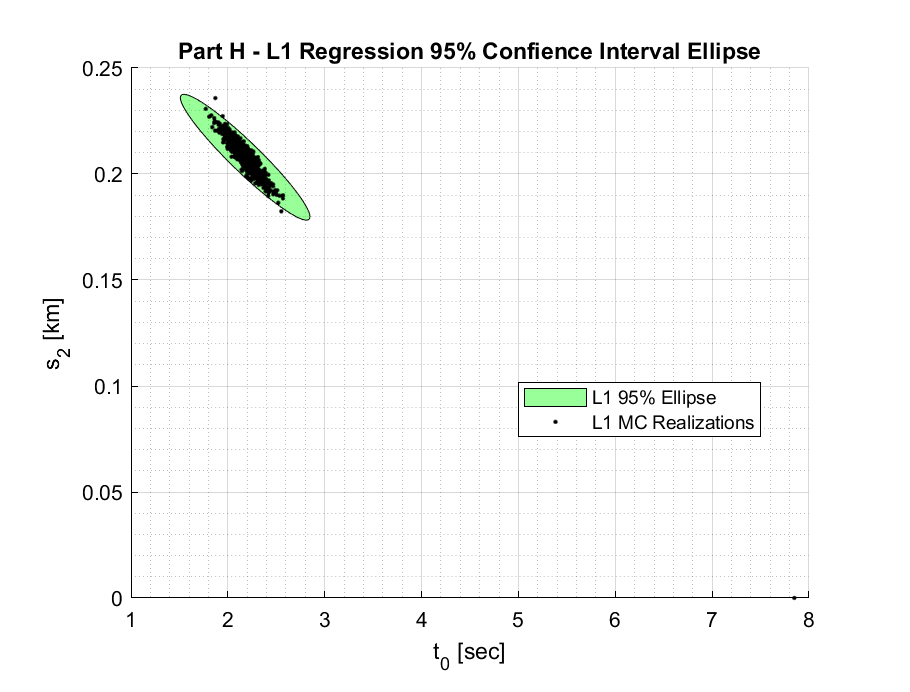
\includegraphics[width=0.8\textwidth]{./images/prob1_partH.eps}
 	\caption{Part H - L1 Monte-Carlo Realizations vs. 95\% Confidence Ellipse}
 	\label{fig: prob1 partH}
 \end{figure}
 \FloatBarrier
 
 Notice that one Monte-Carlo realization sits in the far right-bottom corner.

\subsubsection{Part I}

Recall in figure \ref{fig: prob1 partG} that the L1 regression residuals were all less than the L2 regression residuals for the first 5 data points, but not the 6th. This implies that the L1 regression assigned "greater importance" to the first 5 data points, which signifies that the 6th data point was in fact an outlier. 

